\documentclass[0-main.tex]{subfiles}
\begin{document}


\section{Introduction}
Kinematic and fixed-camera video demonstrations from robot-assisted minimally invasive procedures can be used for surgical skill assessment~\cite{gao2014jigsaws}, development of finite state machines~\cite{kehoe2014autonomous,murali2015learning}, learning from demonstration (LfD)~\cite{reiley2010motion}, and calibration~\cite{mahler2014learning}.
Surgical tasks are often multi-step procedures that have complex interactions with the environment, and as a result, demonstrations are noisy and may contain superfluous or repeated actions \cite{krishnan2015tsc}.
Temporal segmentation of the demonstrations into meaningful contiguous sections facilitates local learning from demonstrations and salvaging good local segments from inconsistent demonstrations.

Manual annotation provides one approach to segmentation (e.g., \cite{hanlearning}); however, as datasets grow, this can become impractical.
Human annotators can also be prone to error by missing segments or applying segmentation criteria inconsistently across a dataset.
There are a number of recent proposals to algorithmically extract segments \cite{calinon2010learning, Niekum2015learning, krishnan2015tsc}.
Such algorithms fall into two broad categories: (1) dictionary-based, (2) and unsupervised.
Dictionary-based algorithms require a pre-defined vocabulary of primitives and decompose new trajectories in terms of the primitives.
However, specific primitives may not cover all of the actions seen in a set of demonstrations, while broad primitives may overlook important transitions.

\begin{figure}[t!]
\centering
\vspace{-5pt}
% 
\includegraphics[width=0.5\linewidth]{figures/insert}
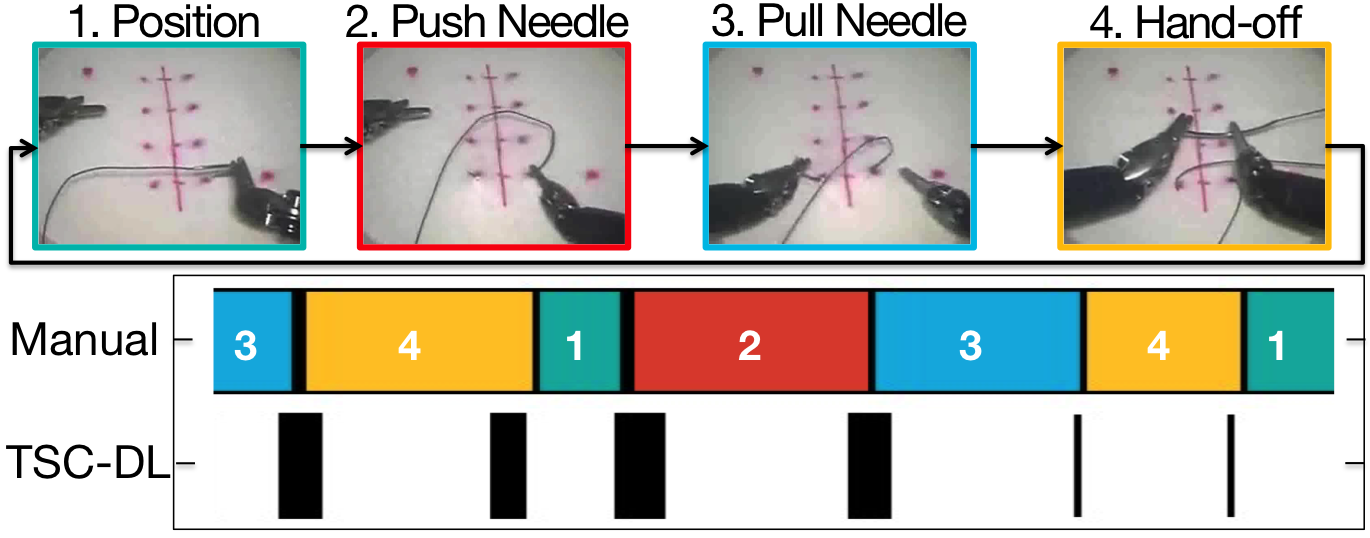
\includegraphics[width=\linewidth]{figures/suturing-teaser-v4.png}
\caption{We apply \tsc to a suturing task. Each ``throw" of suturing repeats between four steps, and figure illustrates that \tsc extracts a segmentation that closely aligns with the manual annotation without supervision.}
\figlabel{surgical-teaser}
% \label{fig:pr2_toyplane}
\vspace{-15pt} 
\end{figure}


% \iffalse
\begin{SCfigure*}[][t!]
    \centering
    \vspace{-10pt}
    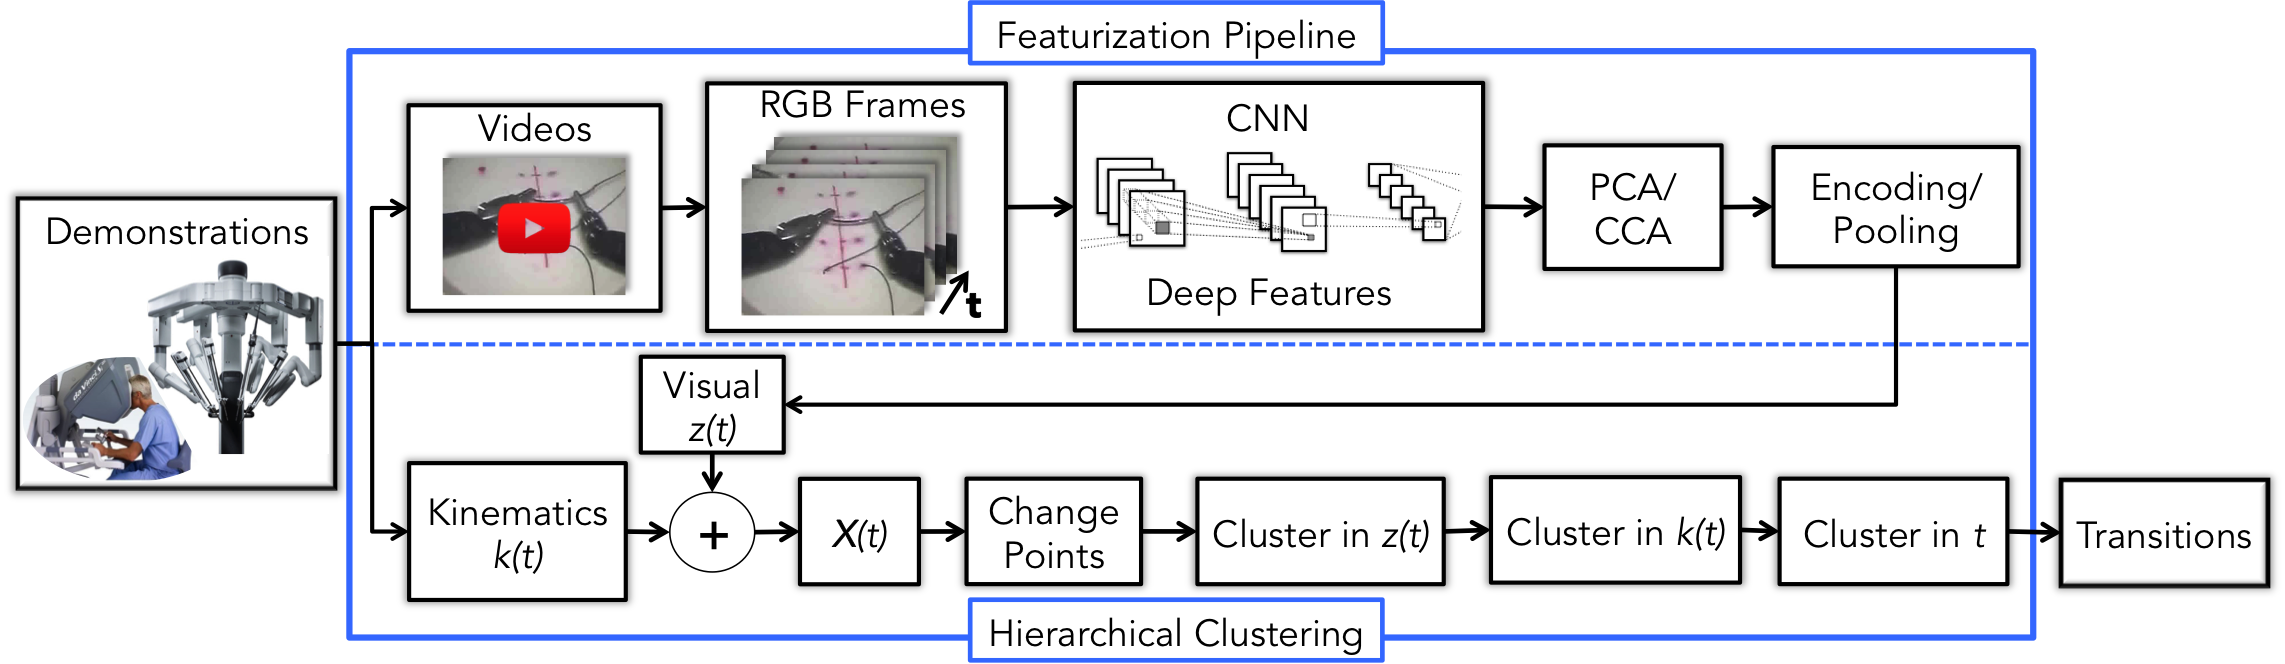
\includegraphics[width=1.55\linewidth]{figures/sysArch}
    \caption{We use a visual processing pipeline with deep features to construct a trajectory of high-dimensional visual states $z(t)$.
    We concatenate encoded versions of these features with kinematics and apply hierarchical clustering to find segments.}%dont add more lines--seems to mess up formatting
    \label{fig:pipeline}
    \vspace{-10pt}
\end{SCfigure*}
% \fi

% \begin{figure*}[!t]
% \centering
% 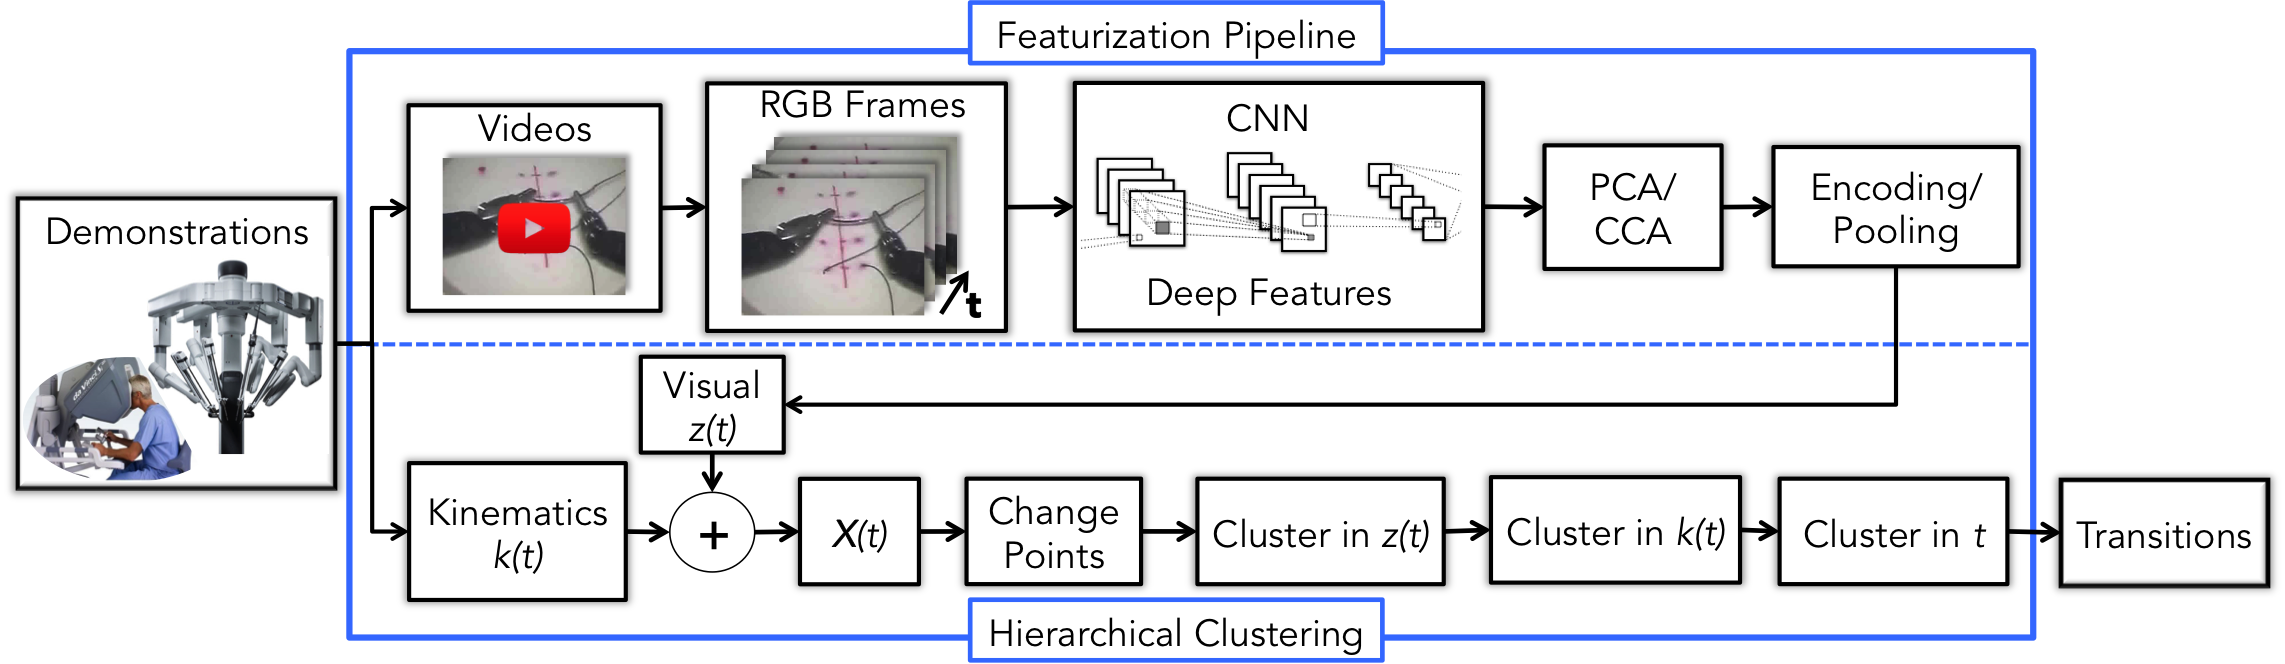
\includegraphics[width=0.8\linewidth]{figures/sysArch}
% \caption{\tsc is a task segmentation pipeline that starts with multimodal demonstrations (kinematics and vision), uses deep learning to featurize the frames of the video, and then clusters transition events to find segments.}
% \label{fig:pipeline}
% \vspace{-15pt}
% \end{figure*}

Unsupervised techniques avoid dependence on a pre-defined set of primitives using generative mixture models for the data, e.g., locally Gaussian segments, and fit trajectories to these models by clustering together locally similar points \cite{calinon2010learning, krishnan2015tsc, kruger2010learning} \del{fox2009nonparametric}.
A clustering model allows us to detect outliers and inconsistencies (segmentation points that lie in small clusters) without annotations susceptible to human error.
It can also give us a natural notion of confidence, through the goodness-of-fit, which can guide the acquisition of demonstrations of segments that require more data. 
While unsupervised segmentation has been widely studied in the context of kinematic data, increasingly, fixed-camera video is also available.

Visual features can provide information about the state of manipulated objects~\cite{krishnan2015tsc, Niekum2015learning}, and trajectory information when there is state-dependent sensor noise in kinematic data \cite{mahler2014learning}.
Existing work uses hand-tuned features~\cite{krishnan2015tsc}, poses for all objects in the workspace via AR markers~\cite{Niekum2015learning}, or motion capture markers~\cite{kulic2011incremental}.
We explore relaxing these constraints by applying recent results in Deep Learning to learn a visual representation that generalizes across tasks.

In this paper, we significantly extend our prior segmentation work, Transition State Clustering~\cite{krishnan2015tsc}, with automatically constructed visual features using \textit{deep} convolutional neural networks (CNNs).
Computer vision frameworks such as CAFFE~\cite{jia2014caffe} can leverage recent advances in CNNs~\cite{krizhevsky2012imagenet, jia2014caffe, long2014fully} through pre-trained models (on large corpora of natural images). 
CNNs learn expressive but general feature representations that transfer across domains allowing us to take advantage of the models without having to acquire a large number of examples. 
Transition State Clustering segments demonstrations by learning switched linear dynamical systems and using clustering to identify regions of the state-space associated with switching events.
TSC applies a Dirichlet Process Gaussian mixture hierarchically first clustering transition states spatially and then temporally.
Our prior results suggested that augmenting the state-space with hand-tuned visual features could significantly improve accuracy.
In the present paper, we extract visual features using filters derived from layers of pre-trained CNNs applied to frames of video recordings and call this new algorithm Transition State Clustering with Deep Learning (\tsc).
This constructs a high-dimensional trajectory that augments the kinematic state-space (Figure \ref{fig:pipeline}).

% In computer vision, the growing maturity of \emph{deep} featurization e.g., Convolutional Neural Networks (CNNs), has led to a number of seminal results in visual feature extraction \cite{krizhevsky2012imagenet, jia2014caffe, long2014fully}.\del{lecun1995convolutional} Furthermore, frameworks like CAFFE \cite{jia2014caffe} allow for sharing pre-trained models (on large corpora of natural images), and this allows us to take advantage of these results even with relatively small datasets.

We study CNN features for unsupervised temporal trajectory segmentation on five datasets: (1) a synthetic 4 segment example, (2) JIGSAWS surgical needle passing, (3) JIGSAWS surgical suturing, (4) toy plane assembly by the PR2, and (5) Lego assembly by the PR2.
On the synthetic example, we find that \tsc recovers the 4 underlying segments in the presence of partial state observation (one kinematic state hidden), control noise, and sensor noise. 
\tsc is an unsupervised algorithm that consistently applies segmentation criteria derived from linear dynamical regimes.
We compare this criteria with manual annotations when available.
On real datasets, we find that \tsc matches the manual annotation with up to 0.806 normalized mutual information.
Our results also suggest that including kinematics and vision results in increases of up-to 0.215 NMI over kinematics alone.
We demonstrate the benefits of using an unsupervised approach by presenting examples where \tsc discovers unlabeled segments due to human annotator error (as shown in Figure \ref{fig:suturing}), and can learn across demonstrations with widely varying operator skill levels (as shown in Table \ref{tab:jigsaws}).


%Clustering allows focussed LFD on each segment resulting in a better fit. 
%Clustering can identify inconsistent outliers and dirty data segments that cann corrupt LFD, also 
%Can identify segments where more consistent data is needed.
%can salvage good segments form bad demo sequences. 

%emph unsupervised
%avoids human bias
%apply consistent models -- can discover subtle transitions
%faster than humans 
  
\iffalse
\begin{figure}[ht]
\centering
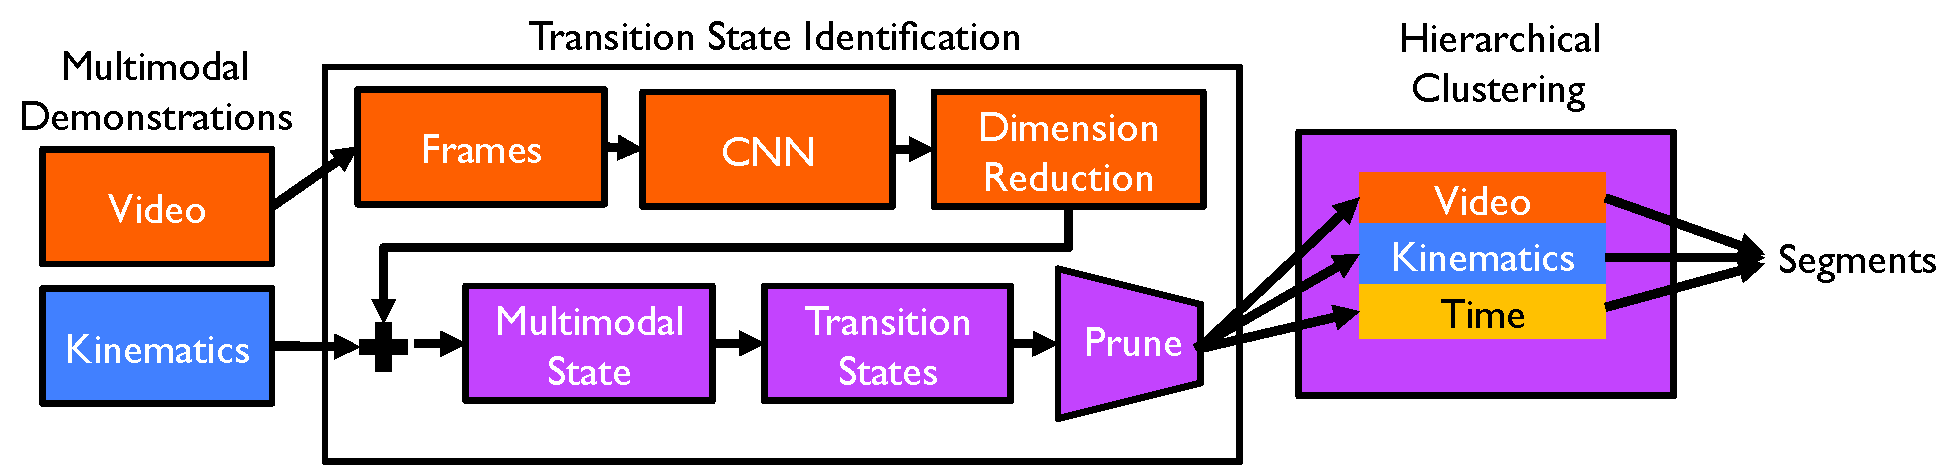
\includegraphics[width=\columnwidth]{figures/architecture.pdf}
\caption{\todo{name} architecture. We use a pre-trained CNN to featurize raw video data for use in segmentation. After featurization, we combine the data with kinematic data and apply a Transition State Clustering algorithm to identify segments.}
\figlabel{arch}
\vspace{-1em}
\end{figure}
\fi

\end{document}